\documentclass[12pt]{report}
\usepackage[utf8]{inputenc}
\usepackage{cite}
\usepackage[hidelinks]{hyperref}
\usepackage{graphicx}
\usepackage{amsfonts}
\usepackage{mathtools}
\usepackage{caption}
\usepackage{fancyhdr}

\pagestyle{fancy}
\fancyhf{}
\rhead{5-stage Pipelined Processor Design Report}
\lhead{\thesection}
\rfoot{\thepage}

\DeclarePairedDelimiter\ceil{\lceil}{\rceil}
\DeclarePairedDelimiter\floor{\lfloor}{\rfloor}

\title{\textbf{5-stage Pipelined Processor Design Report}\\Team \#4}
\author{
  Mohamed Shawky\\
  \small\texttt{SEC:2, BN:16}
  \and
  Remonda Talaat\\
  \small\texttt{SEC:1, BN:20}
  \and
  Evram Youssef\\
  \small\texttt{SEC:1, BN:9}
  \and
  Mahmoud Adas\\
  \small\texttt{SEC:2, BN:21}
}
\date{\today}

\begin{document}

\thispagestyle{empty}

\maketitle
\tableofcontents
\listoffigures
\listoftables
\clearpage

\pagenumbering{arabic}

\part{Introduction}

\section{System Overview}
This document reports our design work of the 5-stage pipelined processor using Harvard
architecture. We discuss the overall system blocks and connections, the functionalities of the
different blocks and the hazard solutions. 

\section{Task Distribution}
\begin{center}
    \captionof{table}{Task Distribution\label{tab:td}}
 \begin{tabular}{||c| p{100mm}||} 
 \hline
 Team Member & Tasks \\ [0.5ex] 
 \hline\hline
 Mohamed Shawky & 1) Overall system design. \newline 2) Hazard detection and handling. \newline 3) Document typing and formatting. \\
 \hline
 Remonda Talaat & 1) Instruction format. \newline 2) Interrupt Handling. \newline 3) Overall system design. \\
 \hline
 Evram Youssef & 1) Control unit and its signals. \newline 2) Low level block design. \newline 3) Pipeline buffers. \\
 \hline
 Mahmoud Adas & 1) Low level block design. \newline 2) Pipeline buffers. \newline 3) Document typing and formatting. \\ 
 \hline\hline
\end{tabular}
\end{center}

\part{Overall System}

\section{Overall System Design Schema}
\begin{center}
    \begin{figure}[hp]
        \centering
        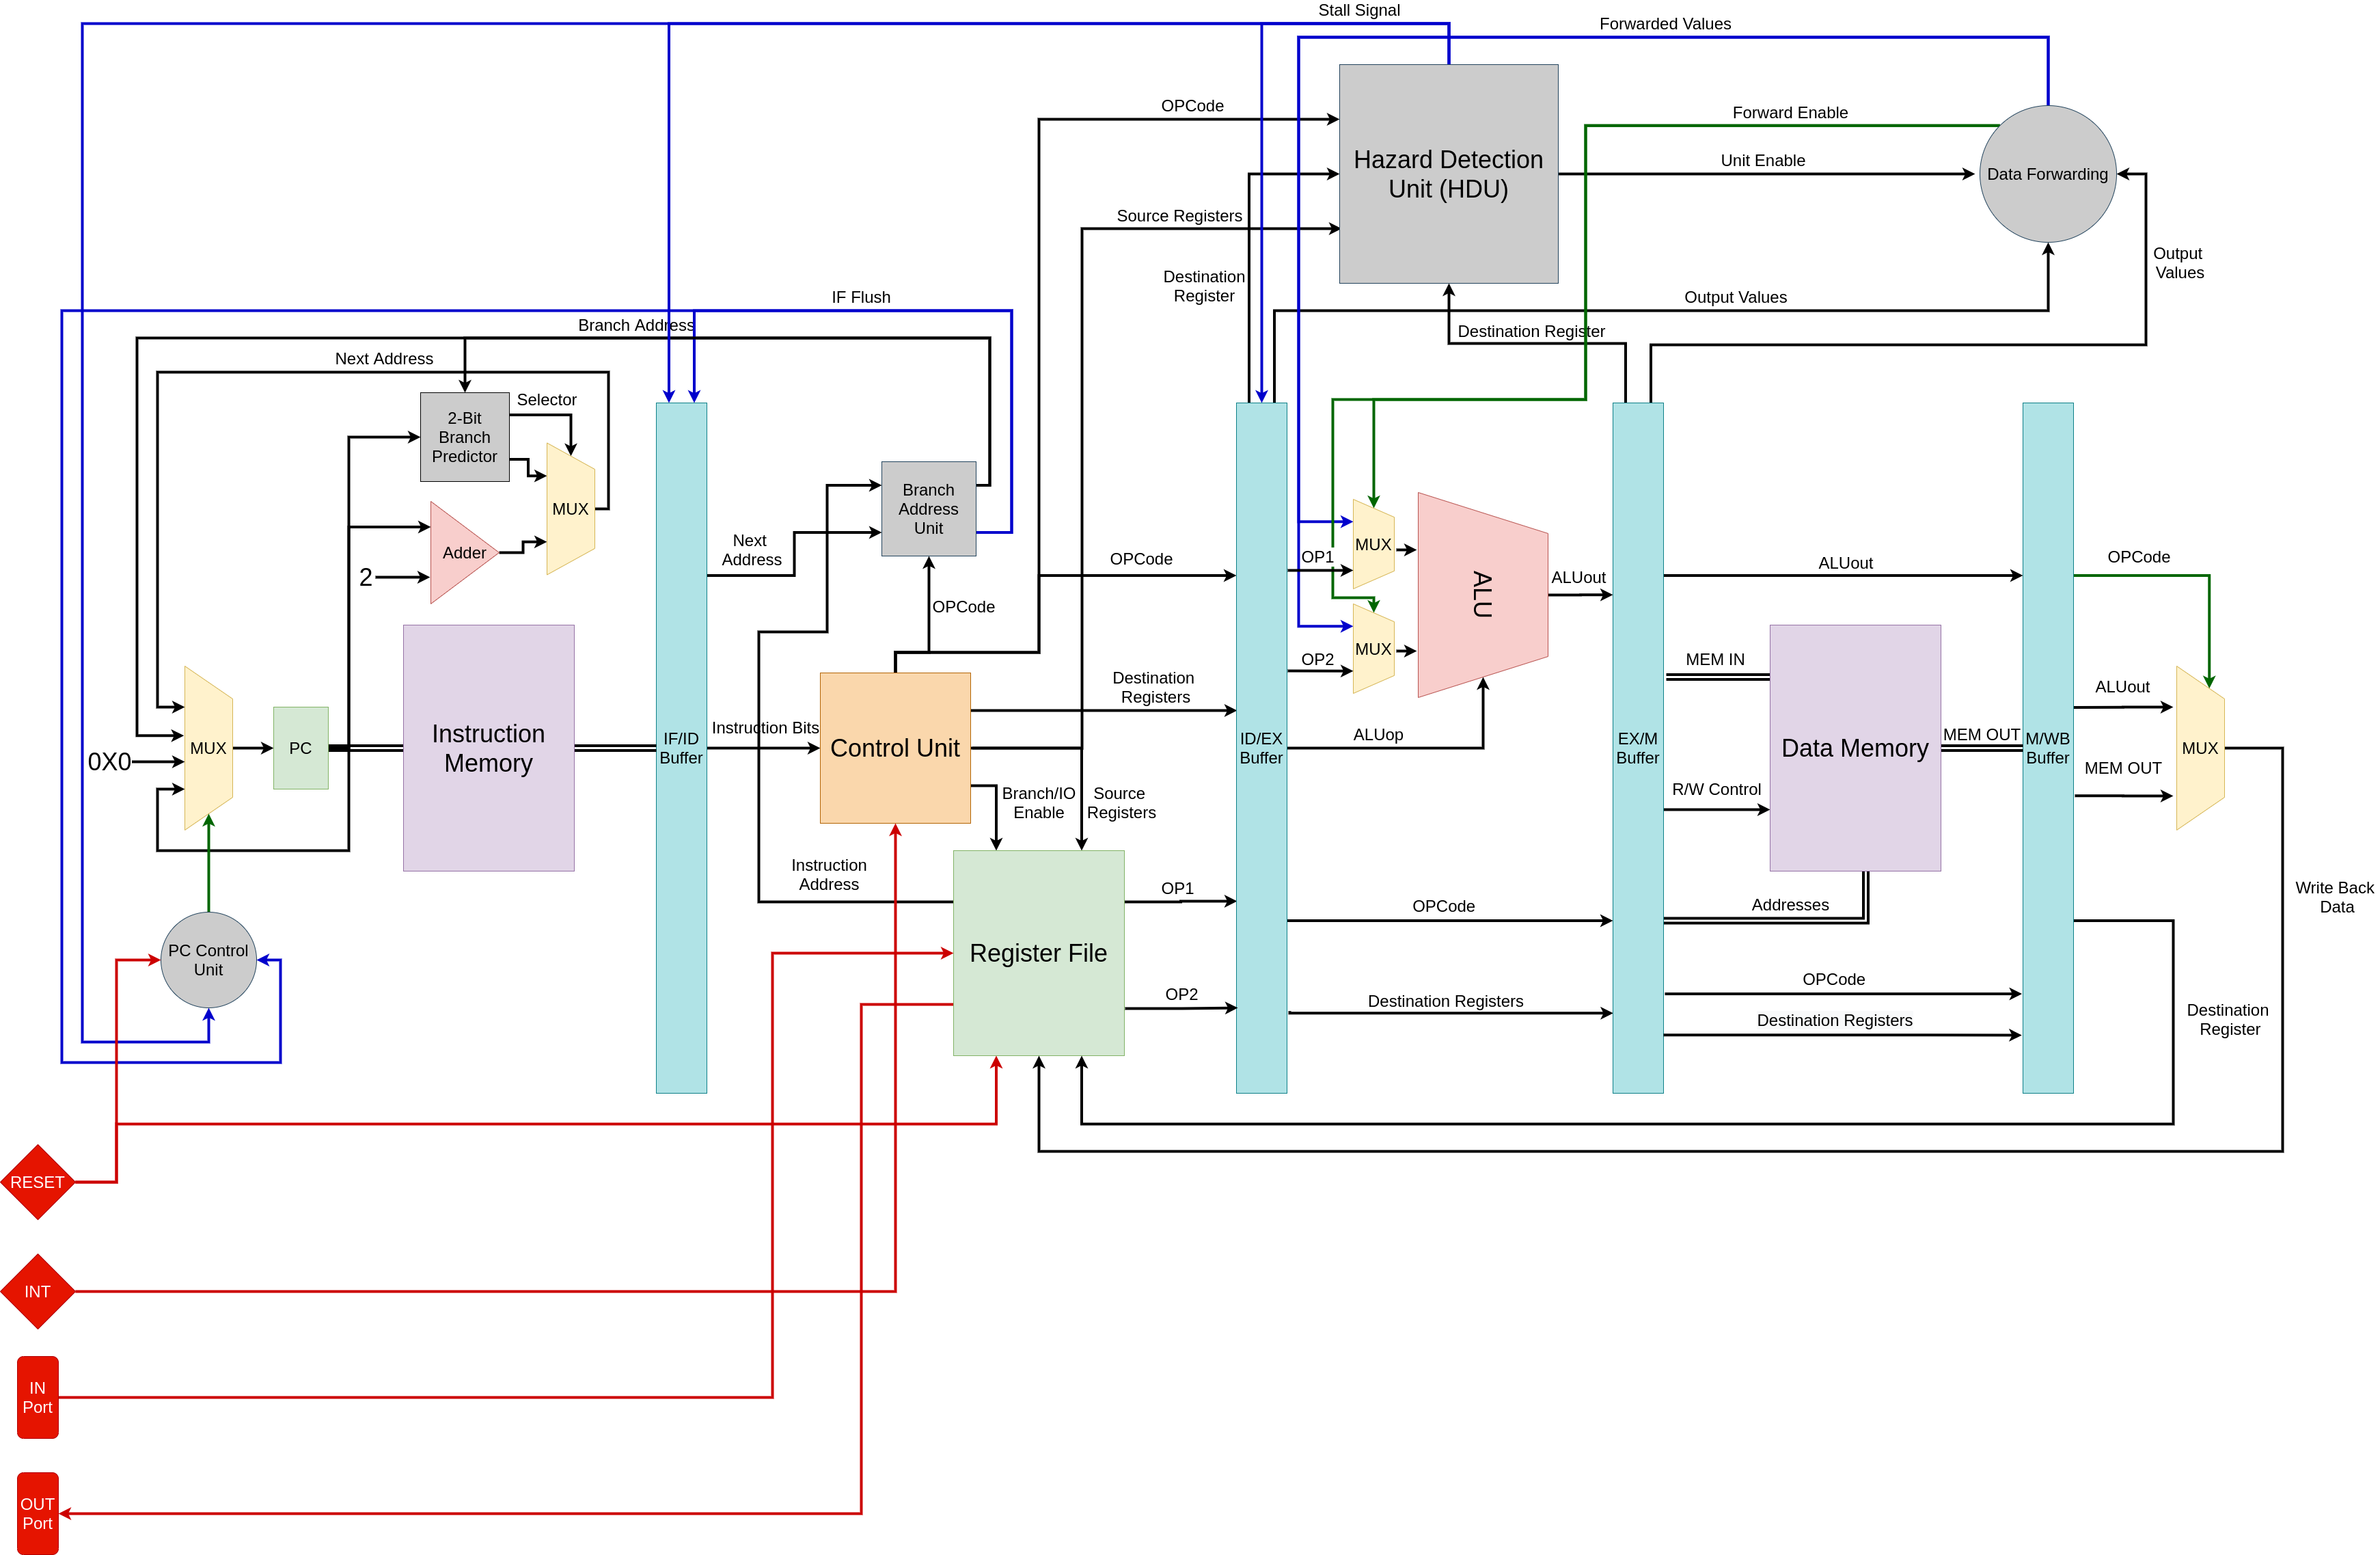
\includegraphics[width=\textwidth]{overall_system}
        \caption{Overall System Design}
        \label{fig:overall}
    \end{figure}
\end{center}

\section{Memory Specs}
\begin{itemize}
    \item We have 2 separate memory units, one for instructions and another for data and stack.
    \item Instruction Memory:
    \begin{itemize}
        \item 2$^{32}$ $X$ 16 bits
        \item 16-bit bus
    \end{itemize}
    \item Data Memory:
    \begin{itemize}
        \item 2$^{32}$ $X$ 16 bits
        \item 32-bit bus
        \item SP starts at 2$^{32}$-1
    \end{itemize}
\end{itemize}

\section{PC Control Unit}

\subsection{Inputs}
\begin{itemize}
    \item IF Flush (1 bit)
    \item Stall Signal (1 bit)
    \item RESET Signal (1 bit)
    \item Interrupt Signal (1 bit)
    \item Current OPCode (7 bits)
\end{itemize}

\subsection{Outputs}
\begin{itemize}
    \item PC Mux Selectors (3 bits)
\end{itemize}

\subsection{Logic}
\begin{itemize}
    \item If IF Flush == 1, Output = 001
    \item If RESET == 1, Output = 010
    \item If Stall == 1, Output = 011
    \item If Interrupt == 1 $||$ OPCode == RET/RTI, Output = 100
    \item Else, Output = 000
\end{itemize}

\begin{center}
    \begin{figure}[hp]
        \centering
        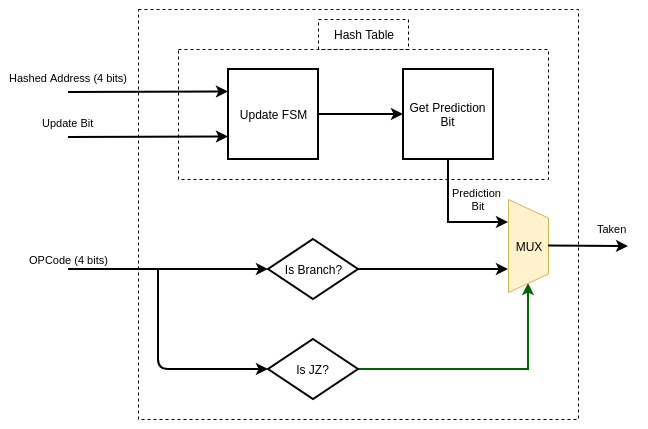
\includegraphics[width=0.8\textwidth]{bpu}
        \caption{Branch Prediction Unit Diagram}
        \label{fig:bpu}
    \end{figure}
\end{center}

\section{Dynamic Branch Prediction}

\subsection{Inputs}
\begin{itemize}
    \item Hashed Address (4 bits)
    \item Update Bit (1 bit): \emph{Taken or Not}  to update FSM
    \item OPcode (4 bits)
\end{itemize}

\subsection{Outputs}
\begin{itemize}
    \item Taken (1 bit): predict whether the branch taken or not
\end{itemize}

\subsection{Logic}
\begin{itemize}
    \item Updates the FSM corresponding to the hashed address.
    \item Checks whether the OPCode is of a conditional branch instruction.
    \item Outputs the prediction bit \emph{(Taken or Not)} accordingly.
\end{itemize}

\begin{center}
    \begin{figure}[hp]
        \centering
        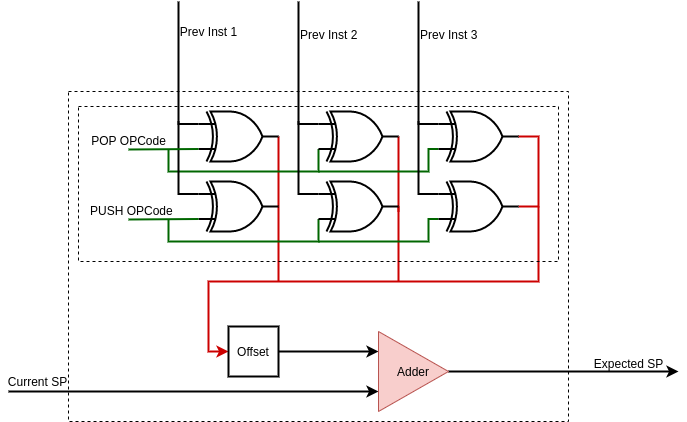
\includegraphics[width=0.8\textwidth]{pspu}
        \caption{Stack Pointer (SP) Peak Unit Diagram}
        \label{fig:pspu}
    \end{figure}
\end{center}

\section{Stack Pointer (SP) Peak Unit}

\subsection{Inputs}
\begin{itemize}
    \item Current SP (32 bits)
    \item Prev OPCodes (3$X$7 bits)
\end{itemize}

\subsection{Outputs}
\begin{itemize}
    \item Expected SP (32 bits): stack pointer to read from after eliminating hazards
\end{itemize}

\subsection{Logic}
This unit peaks the value of the stack pointer on returning from a subroutine or an interrupt, in order to calculate the correct value of the address from which the original program counter read from memory. It checks for \emph{POP/PUSH} instructions and use the count to update the address.\\
\textbf{NOTE:} In case we didn't use this unit, we will stall the pipe for three consecutive cycles to eliminate possible hazards.

\begin{center}
    \begin{figure}[hp]
        \centering
        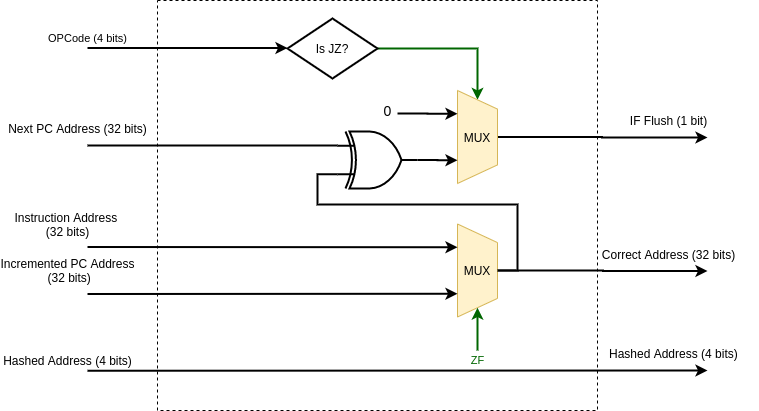
\includegraphics[width=0.8\textwidth]{bau}
        \caption{Branch Address Unit Diagram}
        \label{fig:bau}
    \end{figure}
\end{center}

\section{Branch Address Unit}

\subsection{Inputs}
\begin{itemize}
    \item Next PC Address (32 bits)
    \item Instruction Address (32 bits)
    \item Incremented PC Address (32 bits)
    \item Hashed Address (4 bits)
    \item OpCode (4 bits)
\end{itemize}

\subsection{Outputs}
\begin{itemize}
    \item IF Flush (1 bit)
    \item Branch Address (32 bits)
    \item Hashed Address (4 bits)
\end{itemize}

\subsection{Logic}
\begin{itemize}
    \item Check if OpCode is of a conditional branch instruction, if true:
    \begin{itemize}
        \item Check whether PC Next Address is equal to Instruction Address
        \item If true:
        \begin{itemize}
            \item IF Flush = 0, Branch Address = Instruction Address
        \end{itemize}
        \item If false:
        \begin{itemize}
            \item IF Flush = 1, Branch Address = Instruction Address
        \end{itemize}
    \end{itemize}
\end{itemize}

\begin{center}
    \begin{figure}[hp]
        \centering
        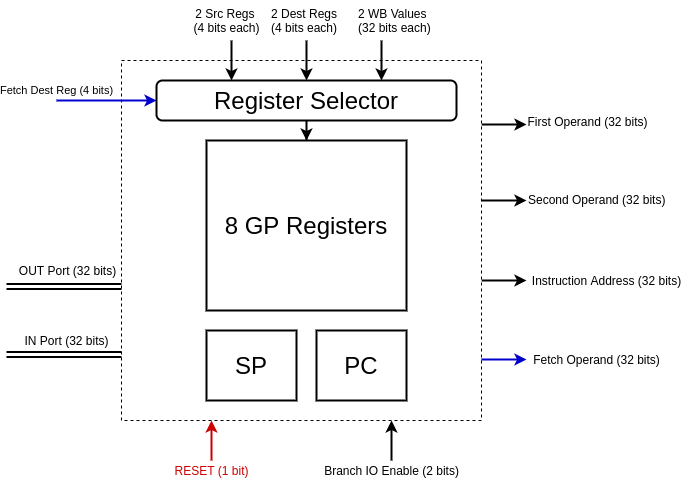
\includegraphics[width=0.8\textwidth]{reg_file}
        \caption{Register File Diagram}
        \label{fig:reg_file}
    \end{figure}
\end{center}

\section{Register File}

\subsection{Registers}
\begin{itemize}
    \item 8 general purpose registers
    \item Stack pointer (SP) register
    \item Program counter (PC) register
\end{itemize}

\subsection{Inputs}
\begin{itemize}
    \item Dest Regs: 2$X$4 bits (for destination selection)
    \item SRC Regs: 2$X$4 bits (for source selection)
    \item Fetch Reg: 4 bits (for fetch branch register selection)
    \item WB values: 2$X$32 bits (for write back values)
    \item RESET: 1 bit (for registers clear).
    \item Branch/IO: 2 bits (to determine whether the operation is IO or branch)
    \item IN Port: 32 bits (IO input port)
\end{itemize}

\subsection{Outputs}
\begin{itemize}
    \item OP1: 32 bits (value of first operand)
    \item OP2: 32 bits (value of second operand)
    \item Fetch Value: 32 bits (value of branch address required by fetch)
    \item Instruction Address: 32 bits (value of branch address)
    \item OUT Port: 32 bits (IO output port)
\end{itemize}

\subsection{Logic}
The register selector acts like a decoder to select the required operation and the register on which the operation performed.

\section{ALU}

\subsection{Inputs}
\begin{itemize}
    \item ALUop: 4 bits (refer to ALU Operations below)
    \item Operands: 2$X$32 bits (2 input operands)
\end{itemize}

\subsection{Outputs}
\begin{itemize}
    \item ALUout: 32 bits (operation result)
\end{itemize}

\subsection{ALU Operations}
\begin{itemize}
    \item 0000 $-$ NOP $-$ (no operation)
    \item 0001 $-$ INC $-$ (first operand + 1)
    \item 0010 $-$ DEC $-$ (first operand - 1)
    \item 0011 $-$ ADD $-$ (first operand + second operand)
    \item 0100 $-$ SUB $-$ (first operand - second operand)
    \item 0101 $-$ AND $-$ (first operand \&\& second operand)
    \item 0110 $-$ OR $-$ (first operand $||$ second operand)
    \item 0111 $-$ NOT $-$ (!first operand)
    \item 1000 $-$ SHL $-$ (shift first operand to the left)
    \item 1001 $-$ SHR $-$ (shift first operand to the right)
    \item 1010 $-$ INC2 $-$ (first operand + 2)
    \item 1011 $-$ DEC2 $-$ (first operand - 2)
    \item 1100 $-$ INC4 $-$ (first operand + 4)
    \item 1101 $-$ DEC4 $-$ (first operand - 4)
\end{itemize}

\subsection{Logic}
\begin{itemize}
    \item ALU performs the operation and changes the CCR accordingly.
    \item The input operands of the ALU are multiplexed between forwarded data and register data, with selectors from data forwarding unit.
\end{itemize}

\part{Instruction Format}

\section{One Operand Operations}
\begin{itemize}
    \item 4 bits (1111) for one operand instructions.
    \item 3 bits to define instruction.
    \item 3 bits for destination register.
    \item 1 bit to define the memory slots occupied by the instruction.
    \item Total of 11 bits, padded with 5 0's to fit 16 bits.
\end{itemize}
\begin{center}
    \captionof{table}{One Operand Instruction Mapping\label{tab:1op}}
 \begin{tabular}{||c| c| c| c| p{40mm}||} 
 \hline
 Operation & OpCode & Destination & 16$|$32 & Conditions  \\ [0.5ex] 
 \hline\hline
 IN & 1111000 & 000:111 & 0 & ----------------------- \\
 \hline
 NOT & 1111001 & 000:111 & 0 & if !Rdst=0,Z=1 \newline if !Rdst$<$0,N=1 \\
 \hline
 INC & 1111010 & 000:111 & 0 & if Rdst+1=0,Z=1 \newline if Rdst+1$<$0,N=1 \\
 \hline
 DEC & 1111011 & 000:111 & 0 & if Rdst-1=0,Z=1 \newline if Rdst-1$<$0,N=1 \\
 \hline
 OUT & 1111100 & 000:111 & 0 & ----------------------- \\
 \hline
\end{tabular}
\end{center}

\section{Special Operations}
\begin{itemize}
    \item 16 0's to represent NOP (0000000000000000).
\end{itemize}

\section{Two Operand Operations}
\begin{itemize}
    \item 4 bits to define instruction.
    \item 3 bits for each of Rsrc1, Rsrc2 and Rdst.
    \item 1 bit to define the memory slots occupied by the instruction.
    \item 16 bits for immediate values.
    \item Total of 14 bits in most cases with some exceptions mentioned below.
\end{itemize}
\begin{center}
    \captionof{table}{Two Operand Instruction Mapping\label{tab:1op}}
 \begin{tabular}{||c| c| c| c| c| c| c| p{30mm}||} 
 \hline
 Operation & OpCode & Rsrc1 & Rsrc2 & Rdst & imm & 16$|$32 & Conditions  \\ [0.5ex] 
 \hline\hline
 SWAP & 0001 & 000:111 & --- & 000:111 & --- & 0 & ----------------------- \\
 \hline
 ADD & 0010 & 000:111 & 000:111 & 000:111 & --- & 0 & if Result=0,Z=1 \newline if Result$<$0,N=1 \\
 \hline
 SUB & 0011 & 000:111 & 000:111 & 000:111 & --- & 0 & if Result=0,Z=1 \newline if Result$<$0,N=1 \\
 \hline
 AND & 0100 & 000:111 & 000:111 & 000:111 & --- & 0 & if Result=0,Z=1 \newline if Result$<$0,N=1 \\
 \hline
 OR & 0101 & 000:111 & 000:111 & 000:111 & --- & 0 & if Result=0,Z=1 \newline if Result$<$0,N=1 \\
 \hline
 SHL & 0110 & 000:111 & --- & --- & 16 bits & 1 & update carry flag \\
 \hline
 SHR & 0111 & 000:111 & --- & --- & 16 bits & 1 & update carry flag \\
 \hline
 IADD & 1000 & 000:111 & --- & 000:111 & 16 bits & 1 & if Result=0,Z=1 \newline if Result$<$0,N=1 \\
 \hline
\end{tabular}
\end{center}

\section{Memory Operations}
\begin{itemize}
    \item 4 bits to define instruction.
    \item 3 bits for destination register.
    \item 1 bit to define the memory slots occupied by the instruction.
    \item 16 bits for immediate values.
    \item 20 bits for effective addresses.
    \item Total of 8 bits with no immediate values or effective addresses.
    \item Total of 24 bits with immediate values.
    \item Total of 28 bits with effective addresses.
\end{itemize}
\begin{center}
    \captionof{table}{Memory Instruction Mapping\label{tab:1op}}
 \begin{tabular}{||c| c| c| c| c| c| p{40mm}||} 
 \hline
 Operation & OpCode & Rdst & imm & EA & 16$|$32 & Conditions  \\ [0.5ex] 
 \hline\hline
 PUSH & 1001 & 000:111 & --- & --- & 0 & ----------------------- \\
 \hline
 POP & 1010 & 000:111 & --- & --- & 0 & ----------------------- \\
 \hline
 LDM & 1011 & 000:111 & 16 bits & --- & 1 & ----------------------- \\
 \hline
 LDD & 1100 & 000:111 & --- & 20 bits & 1 & ----------------------- \\
 \hline
 STD & 1101 & 000:111 & --- & 20 bits & 1 & ----------------------- \\
 \hline
\end{tabular}
\end{center}

\section{Branch and Change Control Operations}
\begin{itemize}
    \item 4 bits (0000) for branching instructions.
    \item 3 bits to define instruction.
    \item 3 bits for destination register.
    \item 1 bit to define the memory slots occupied by the instruction.
    \item Total of 11 bits, padded with 5 0's to fit 16 bits. 
\end{itemize}
\begin{center}
    \captionof{table}{One Operand Instruction Mapping\label{tab:1op}}
 \begin{tabular}{||c| c| c| c| p{40mm}||} 
 \hline
 Operation & OpCode & Destination & 16$|$32 & Conditions  \\ [0.5ex] 
 \hline\hline
 JZ & 0000001 & 000:111 & 0 & ----------------------- \\
 \hline
 JMP & 0000010 & 000:111 & 0 & ----------------------- \\
 \hline
 CALL & 0000011 & 000:111 & 0 & ----------------------- \\
 \hline
 RET & 0000100 & --- & 0 & ----------------------- \\
 \hline
 RTI & 0000101 & --- & 0 & ----------------------- \\
 \hline
\end{tabular}
\end{center}

\part{Control Signals}

\section{Overview}
Control unit is responsible for generating the control signals that are used to activate several operations throughout the pipeline. Also, it's responsible for the extraction of specific information from instruction bits.
\begin{itemize}
    \item Immediate values (16 bits)
    \item Effective addresses (20 bits)
    \item source registers (4 bits)
    \item destination registers (4 bits)
    \item OPCode (4:7 bits)
    \item Branch/IO Enable (2 bits)
    \item ALUop (4 bits)
    \item Interrupt Enable (1 bit)
    \item Memory R/W Enable (2 bits)
    \item second operand selector (1 bit)
\end{itemize}

\textbf{TODO: Add related control signals for each instruction}

\part{Pipeline Stages}

\section{Overview}
This section discusses the 5 stages of our system and their functionalities.

\subsection{Fetch Stage}
\begin{itemize}
    \item Responsible for fetching the next instruction.
    \item Can take two cycles in case of 32-bit instructions.
    \item Contains a branch prediction unit to determine the next address to be fetched in case of branching.
    \item Outputs the instruction bits into IF/ID Buffer.
    \item The current instruction is fetched at the first half of cycle, then the next PC value calculations are done in the second half.
\end{itemize}

\subsection{Decode Stage}
\begin{itemize}
    \item Responsible for decoding the instruction bits into control signals.
    \item Outputs the corresponding signals to ID/EX Buffer.
    \item Contains register file to output operand values and register-related operations.
    \item Determines the correct branch address in case of branching instructions by using Branch Address Unit.
    \item The control unit deduces the corresponding signals in the first half of cycle, then the register operations and branch address calculation are done in the second half of cycle.
\end{itemize}

\subsection{Execute Stage}
\begin{itemize}
    \item Responsible for ALU operations.
    \item Determines the correct ALU output and pass it with other signals to EX/M Buffer.
    \item The ALU operations and CCR update are done in the first half of cycle.
\end{itemize}

\subsection{Memory Stage}
\begin{itemize}
    \item Responsible for Data Memory IO.
    \item Memory read/write is done in the first half of cycle.
\end{itemize}

\subsection{Write-Back Stage}
\begin{itemize}
    \item Responsible for passing correct output values to the destination registers.
    \item Write back is done in the first half of cycle.
\end{itemize}

\section{IF/ID Buffer}

\subsection{Registers}
\begin{itemize}
    \item Instruction Register (32 bits)
    \item Next Address Register (32 bits)
    \item Incremented PC Register (32 bits)
    \item Hashed Address Register (4 bits)
    \item Interrupt Register (1 bit)
\end{itemize}

\subsection{Control Signals}
\begin{itemize}
    \item Flush: clear buffer (1 bit)
    \item Stall: freeze buffer (1 bit)
\end{itemize}

\section{ID/EX Buffer}

\subsection{Registers}
\begin{itemize}
    \item Operand Registers (2$X$32 bits)
    \item Destination Register (4 bits)
    \item OpCode Register (7 bits)
    \item R/W Register (2 bits)
\end{itemize}

\subsection{Control Signals}
\begin{itemize}
    \item Stall (IN): freeze buffer (1 bit)
    \item Destination Register (OUT) (4 bits)
    \item Output Values (OUT) (32 bits)
\end{itemize}

\section{EX/M Buffer}

\subsection{Registers}
\begin{itemize}
    \item ALUout Register (32 bits)
    \item MEM IN Register (32 bits)
    \item Opcode Register (7 bits)
    \item Destination Register (4 bits)
    \item R/W Register (2 bits)
\end{itemize}

\subsection{Control Signals}
\begin{itemize}
    \item Destination Register (OUT) (4 bits)
    \item Output Values (OUT) (32 bits)
\end{itemize}

\section{M/WB Buffer}

\subsection{Registers}
\begin{itemize}
    \item ALUout Register (32 bits)
    \item MEM OUT (32 bits)
    \item OpCode (7 bits)
    \item Destination Register (4 bits)
\end{itemize}

\part{Pipeline Hazards and solutions}

\section{Structural Hazards}

\subsection{Detection}
The structural hazard occurs in data memory and register file.

\subsection{Handling}
The structural hazard in data memory is solved by using 2 memory units, one for instructions and one for data. Both have the same specs \emph{(previously mentioned)}. \\
However structural hazard in register file is handled by forcing the write back to happen in the first half of the clock cycle and the decode to happen in the second half.

\section{Data Hazards}
\begin{center}
    \begin{figure}[hp]
        \centering
        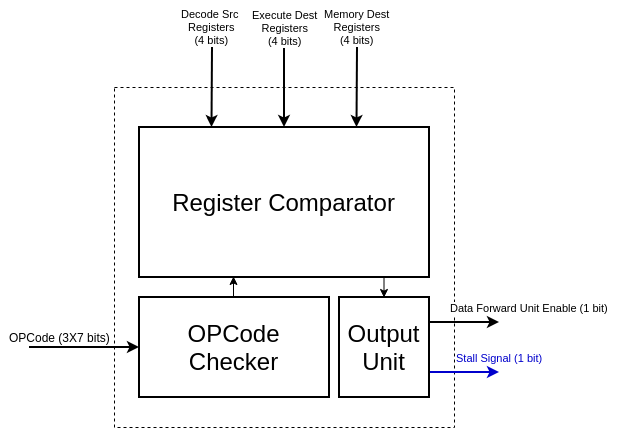
\includegraphics[width=0.8\textwidth]{hdu}
        \caption{Hazard Detection Unit Diagram}
        \label{fig:hdu}
    \end{figure}
\end{center}

\subsection{Detection}
\subsubsection{Hazard Detection Unit (HDU)}
HDU consists of 3 parts:
\begin{itemize}
    \item \textbf{OPCode Checker:} checks the opcode of the current instruction to check whether it will cause data hazard or not, then activates the Register Comparator accordingly. Also, it checks for \emph{load-use case}, in order to activate the stall signal.
    \item \textbf{Register Comparator:} compares the decode source registers with the destination registers of the execute and memory stages.
    \item \textbf{Output Unit:} outputs stall signal in case of load and pop instructions and data forward unit enable in case of other data hazards.
\end{itemize}

\subsection{Handling}

\subsubsection{Stall}
Occurs only at Fetch and Decode stage, due to load(pop) use case.
\begin{itemize}
    \item Fetch same instruction (don't increment the program counter).
    \item Latch IF/ID buffer with the same values.
    \item Freeze Decode stage.
    \item Clear ID/EX buffer.
\end{itemize}

\subsubsection{Data Forwarding}
\begin{itemize}
    \item EX/MEM buffer $->$ Execute / Decode.
    \item ID/EX buffer $->$ Decode.
\end{itemize}

\section{Control Hazards}

\subsection{Detection}
The branch address calculation occurs in the Decode stage. So, the hazard might affect only the Fetch stage, which will be flushed in case of wrong address prediction.

\subsection{Handling}
\begin{itemize}
    \item At Fetch stage, always check the branch predictor and calculate the next address accordingly.
    \item At Decode stage, we have a \emph{Branch Address Unit} that checks whether the OPCode is of a branch operation. If so, it passes the address to the program counter and compares the correct address with the address of the counter to decide whether to flush the Fetch stage or not. 
\end{itemize}

\subsubsection{Flush}
Occurs only at Fetch Stage, due to wrong branch prediction at Decode stage.
\begin{itemize}
    \item Load new address in the program counter.
    \item Remove fetched instructions from IF/ID buffer.
\end{itemize}

\subsubsection{Dynamic Branch Prediction}
We use 2-bit branch predictor, which is a hash table of \emph{Finite State Machines} (FSMs) to predict whether the branch will be taken (1) or not (0) at each individual branch address.

\end{document}
